\documentclass[11pt,answers]{exam}

\usepackage{etex}
\usepackage{amssymb,amsmath,multicol} %<-- InWorksheetExam1 i also have fancyhdr,

\usepackage{hyperref}


\usepackage[metapost]{mfpic}
\usepackage[pdftex]{graphicx}

\usepackage{pst-plot}
\usepackage{pgfplots}
\pgfplotsset{compat=1.9}

\usepackage{tikz}
\usepackage{tkz-2d}
\usepackage{tkz-base}
\usetikzlibrary{calc}

\usepackage[inline]{enumitem}
\usepackage{refcount}%<-- non in WorksheetExam1
\usepackage{subcaption}

\usepackage{tabularx, booktabs}

\newcommand*\circled[1]{\tikz[baseline=(char.base)]{%
		\node[shape=circle,draw,inner sep=1pt] (char) {#1};}}
\renewcommand\choicelabel{\circled{\thechoice}}

\newcommand*\squared[1]{\tikz[baseline=(char.base)]{%
		\node[shape=rectangle,fill=green!20,draw,inner sep=3pt] (char) {#1};}}


\let\originalleft\left
\let\originalright\right
\renewcommand{\left}{\mathopen{}\mathclose\bgroup\originalleft}
\renewcommand{\right}{\aftergroup\egroup\originalright}

%\qformat{\bf{\thequestion}}
%\renewcommand{\headrulewidth}{0pt}

\newcommand{\vasymptote}[2][]{
    \draw [densely dashed,#1] ({rel axis cs:0,0} -| {axis cs:#2,0}) -- ({rel axis cs:0,1} -| {axis cs:#2,0});
}

\makeatletter
\newcommand{\inlineitem}[1][]{%
\ifnum\enit@type=\tw@
    {\descriptionlabel{#1}}
  \hspace{\labelsep}%
\else
  \ifnum\enit@type=\z@
       \refstepcounter{\@listctr}\fi
    \quad\@itemlabel\hspace{\labelsep}%
\fi}
\makeatother

\renewcommand{\questionlabel}{\squared{\thequestion}}

%\qformat{\circled{\thequestion}}

\addpoints
%\printanswers
\noprintanswers

\opengraphsfile{Exam2A_Spring_16}

\begin{document}
\extrawidth{-0.3in}
\pagestyle{headandfoot}

\setlength{\hoffset}{-.25in}

\extraheadheight{-.4in}
\runningheadrule
\firstpageheader{\bfseries {MATH1-UC 1171}}{ \bfseries {Exam 2 }}{\bfseries {5/10/2016}} 



\firstpagefooter{\bfseries{}}{}{} 


\runningheader{\bfseries {}}%
              {\bfseries {}}%
              {Page \thepage\ 
							of \numpages 
							}
\runningfooter{} %%&&CHANGED
                {}
                {Points earned: \hbox to 0.5in{\hrulefill}
                 out of  \pointsonpage{\thepage} points}
                 
						

\vspace*{0.2cm}
\hbox to \textwidth { \scshape {Name:} \enspace\hrulefill}
\vspace{0.2in}

\begin{itemize}
	\item This exam contains \numpages\ pages, including this cover page, the unit circle page and the blank last page which you can tear out and use as scrap paper. Enter
your name on the top of this page, and put your initials
on the top of every page. Please note that I will not grade anything that you write on the last (blank) page.

%\item Please read the instructions for each individual problem carefully. Try not to overthink a problem and read between the lines! Take your time to solve each problem, and don't rush to finish!
%\item Write legibly and clearly label your answers. If I cannot read your solution to a problem, the problem will receive a score of zero.
\item Calculators may not be used in this exam. You may use your note-card with fomulas/examples. 

\item Please write your name on your note-card and include it in your exam. If you do not have a note-card, please write {\textit {no note-card}} on this page.
\item Turn off all phones and computers, and remove all headphones.
\item Cheating is a violation of the SPS policy on academic integrity. The SPS statement on academic integrity and
plagiarism is available at \url{http://tinyurl.com/ko3f79s}. The academic integrity disciplinary procedures outlined on the
website will be strictly enforced.

\end{itemize}

For the problems where you are required to show your work, the following rules apply:\\

\begin{minipage}[t]{3.7in}
\vspace{0pt}
\begin{itemize}

\item \textbf{Include explanations in complete sentences or step-by-step calculations}. If you draw a graph, you must label the axes, include tick marks and include units both on the horizontal and vertical axis. If you are asked to explain in practical terms, then your explanation cannot contain math symbols or formulas.
\item \textbf{Use the methods described in this course} as part of your explanations: for example, you cannot use derivatives to find the peaks and valley of a function.

\item \textbf{Organize your work}, neatly and legibly in
the space provided. Work that is disorganized and difficult to read will not receive full credit.  

\item \textbf{A correct answer, unsupported by calculations, explanation,
or algebraic work will receive no credit}; an incorrect answer supported
by  calculations and explanations may receive
partial credit.


\item \textbf{If you need more space}, use the back of the pages; clearly indicate when you have done this.
\end{itemize}

Do not write in the table to the right.
\end{minipage}
\hfill
\begin{minipage}[t]{2.3in}
\vspace{0pt}
%\cellwidth{3em}
\gradetablestretch{2}
\vqword{Pages}
\addpoints % required here by exam.cls, even though questions haven't started yet.	
\combinedgradetable[v][pages]  % Use [pages] to have grading table by page instead of question

\end{minipage}
\newpage

%\bigskip

%\begin{center}
%\gradetable[v][pages]
%\end{center}

%\newpage

\pointpoints{point}{points}

\begin{questions}


\addpoints
%\qformat{Question \thequestion\dotfill
%         {(\pointsofquestion{\arabic{question}} \points)}}

%\bonusqformat{Bonus Question \thequestion\dotfill
%         {(\bonuspointsofquestion{\arabic{question}} \points)}}        
        
%%%%%%%%%%%%%%%%

\bonusquestion[1]  A principal of 
\$100,000 is deposited in an account that pays an interest of 1\%, compounded yearly. Approximately after how many years will the value of the investment double? Circle the one best answer.
\begin{oneparchoices}
\choice 30
\choice 35
\choice 50
\choice 70
\choice 100
\end{oneparchoices}
\question Decide whether each of the statements listed below is true or false.
\begin{parts}
\part[1] $\displaystyle \log\left ( 2x^3\right )=3\log\left (2x\right)$
\begin{oneparchoices}
\choice True
\choice False
\end{oneparchoices}
\part[1] $\displaystyle \log \left (10^x\right )= x $.
\begin{oneparchoices}
	\choice True
	\choice False
\end{oneparchoices}
\part[1] $\displaystyle \log \left (\frac{1}{2}\right )= -\log (2) $.
\begin{oneparchoices}
\choice True
\choice False
\end{oneparchoices}
%\part[1] $\displaystyle \sqrt[3]{\ln x}=\ln \left (\root[3]{x}\right )$

\part[1] $\displaystyle \sin^{-1}\left (\frac{1}{2}\right ) = \frac{\pi}{6}$.
\begin{oneparchoices}
\choice True
\choice False
\end{oneparchoices}
\part[1] $\displaystyle \sin^{-1}\left (-\frac{1}{2}\right ) = \frac{11\pi}{6}$.
\begin{oneparchoices}
	\choice True
	\choice False
\end{oneparchoices}
%\part[1] $\displaystyle \sin^{-1}\left (\frac{\pi}{2}\right ) = 1$.
%\begin{oneparchoices}
%	\choice True
%	\choice False
%\end{oneparchoices}

\part[1] $\displaystyle \cos(\pi )=-1$.
\begin{oneparchoices}
\choice True
\choice False
\end{oneparchoices}
\end{parts}

\question[2] Evaluate
$f(-1)$ for the function
$\displaystyle f(x) = -\log(99-x)$. Simplify your answer as much as possible. \dotfill
\question The function $g(x)$ is defined by the formula: $\displaystyle g(x) = -2^{x-1} + 2$. 
\begin{parts}
	\part[1] Write the domain of $g(x)$ in interval form. \dotfill
	\part[2] What transformations must be applied to $f(x)=2^x$ to get $g(x)$?
	\fillwithdottedlines{2cm}
	\part[1] Write the range of $g(x)$ in interval form. \dotfill
	
\end{parts}
\bonusquestion[1] A table of value for the periodic function $f(t)$ is shown below. 

\begin{minipage}{\linewidth}
	\centering
	%\captionof{table}{} %\label{tab:title} 
	\begin{tabularx}{0.8\textwidth}{|X|X|X|X|X|X|X|X|X|X|X|X|X|}
		\hline
		\multicolumn{2}{|c|}{$t$}         &0&1& 2 & 3 & 4 & 5 & 6 & 7 &8&9&10\\ \hline
		\multicolumn{2}{|c|}{$f(t)$}   & 12&13 & 14    &12     &13     &14     &12     &13&14 &12 & 13    \\ \hline
	\end{tabularx}
\end{minipage} 
\smallskip

What is the period of the function? \dotfill

\question  The world population grows at a yearly rate of 1.13\% (so every year, the population is 1.13\% larger than the population the previous year.)
\begin{parts}
	%%\part[1] Use the rule of 70 to find the approximate doubling time of the population. 
	
	%%\dotfill
	
	\part[2] Write an equation that you can use to find the number of years it takes the population to increase by 30\%. Explain how you arrive at the equation, but do not  solve it. 
	
	\fillwithdottedlines{2cm}
	
	\part[1] The Earth's population is 7.4 billion people. Assuming a population growth of 1.13\% per year, write a formula that gives the size of the population in 100 years. 
	
	\dotfill
	
\end{parts}

 \question The graph of two periods of a trigonometric function  is shown below:

\begin{mfpic}[35][50]{0}{5.25}{-1.15}{1.5}
%\point[3pt]{(1.5708,0), (2.3562,1), (3.1415,0), (3.927,-1), (4.7124,0)}
\axes
\tlabel[cc](5.25,-0.25){$x$}
\tlabel[cc](0.25,1.5){$y$}
\xmarks{1.5708, 2.3562, 3.1415, 3.927, 4.7124}
\ymarks{-1,1}
\tlpointsep{4pt}
\axislabels {x}{{$\frac{\pi}{2}$} 1.5708, {$\frac{3\pi}{4}$} 2.3562, {$\pi$} 3.1415, {$\frac{5\pi}{4}$} 3.927, {$\frac{3\pi}{2}$} 4.7124}
\axislabels {y}{{$-1$} -1, {$1$} 1}
\function{1.5708, 4.7124, 0.1}{sin(4*x - 1.5708)}
\end{mfpic}

\begin{parts}
\part[2] The amplitude is: \hbox to 1in{\dotfill} The period is: \hbox to 1in{\dotfill}
\part[3]  Write  an equation that represents the curve in the form
$\displaystyle y = a \sin k(x - b)$ or $\displaystyle y = a \cos k(x - b)$. Explain how you find $a$, $k$ and $b$, and write your equation in the space provided below.


\fillwithdottedlines{0.8in}

The equation is $y=$\dotfill
\bonuspart[1]  Redo the problem for the graph shown below.



\begin{mfpic}[35][50]{0}{5.25}{-1.15}{1.5}
%\point[3pt]{(1.5708,0), (2.3562,1), (3.1415,0), (3.927,-1), (4.7124,0)}
\axes
\tlabel[cc](5.25,-0.25){$x$}
\tlabel[cc](0.25,1.5){$y$}
\xmarks{1.5708, 2.3562, 3.1415, 3.927, 4.7124}
\ymarks{-1,1}
\tlpointsep{4pt}
\axislabels {x}{{$\frac{1}{2}$} 1.5708, {$\frac{3}{4}$} 2.3562, {$1$} 3.1415, {$\frac{5}{4}$} 3.927, {$\frac{3}{2}$} 4.7124}
\axislabels {y}{{$-1$} -1, {$1$} 1}
\function{1.5708, 4.7124, 0.1}{sin(4*x - 1.5708)}
\end{mfpic}

\fillwithdottedlines{0.4in}

The equation is $y=$\dotfill

\end{parts}


\question 
\begin{parts}
\bonuspart[1] Is the function $\displaystyle y=\cos^{-1}(x)$ the same as the function $\displaystyle y=\frac{1}{\cos x}$?
\begin{oneparchoices}
\choice Yes \choice No
\end{oneparchoices}
\part[2] The domain of $\displaystyle f(x)=\cos^{-1}(x)$ (in interval form) is \hbox to 1in{\dotfill}
\part[2] The range of $\displaystyle f(x)=\cos^{-1}(x)$ (in interval form) is \hbox to 1in{\dotfill} 
\part[2] Restrict the domain of the function $\displaystyle y=\sin (x)$ to the interval $[0,2\pi]$. Find two different inputs that have the same output. 
\fillwithdottedlines{2cm}

\end{parts}

\question A Ferris wheel with 10 capsules has a diameter of 32 meters and its lowest point (at the 6 o'clock position) is 2 meters above the ground. One full rotation of the wheel takes 12 minutes, and the wheel rotates counterclockwise at a constant speed. The capsules are labeled from 1 to 10. We start observing when capsule 1 is at the 3 o'clock position on the wheel. 
 Let $H(t)$ be the height of capsule 1 $t$ minutes after we start the observation. 
\begin{parts}
\part[2] \label{part:partettob} On the grid provided below, draw the graph of $H(t)$ for $\displaystyle 0\leq t \leq 12$. Label the tick marks on the horizontal and vertical axes.
	
	
	
\begin{tikzpicture}
	\draw[gray!70, thin, step=0.5] (-7,-3) grid (7,3);
	\end{tikzpicture}
\part[1] The amplitude of the graph in part (\ref{part:partettob}) is: \hbox to 1in{\dotfill} \part[1] The period of the graph in part (\ref{part:partettob}) is: \hbox to 1in{\dotfill}
\part[1] The equation of the midline of the graph in part (\ref{part:partettob}) is: \hbox to 1in{\dotfill}
\part[3] During the first rotation of the wheel, at what time(s) is capsule 1 at a height of 10 meters above the ground?
\fillwithdottedlines{3.5cm}
\end{parts}
\question 	A yam has been taken out of an oven and left on a counter at room temperature. The temperature of the yam is $x$ (in degrees Fahrenheit) and the time it takes the yam to reach a temperature of $x$ degrees is $\displaystyle T(x)=745-157\ln\left ( x-60 \right)$ (in minutes). 
	\begin{parts}
		\part[2] What is the initial temperature of the yam, that is, the temperature right after it is taken out of the oven? Explain your reasoning.
	\fillwithdottedlines{2cm}	
		\bonuspart[2] What is the room temperature? Explain your reasoning.
		\fillwithdottedlines{2cm}	
\end{parts}
\newpage
\question A cork floating in a lake is bobbing in simple harmonic motion. Its displacement above the bottom of the lake is modeled by
$\displaystyle y = 0.2 \cos (18\pi t) + 7$
where $y$ is measured in meters and $t$ is measured in minutes.
\begin{parts}
\part[2] On the grid provided below, draw the graph of $y$ (note that $t\geq 0$). Label the tick marks on the horizontal and vertical axes.


\begin{tikzpicture}
	\draw[gray!70, thin, step=0.5] (-7,-3) grid (7,3);
	\end{tikzpicture}
	
\part[1] Find the maximum displacement of the cork above the lake bottom.
	
	\dotfill

\end{parts}
\question[2] The population of a certain city was 171,000 in 2006, and the observed doubling time for the population is 18 years. Find an exponential model 
$\displaystyle n(t) = n_02^{\frac{t}{a}}$
 for the population t years after 2006.
 
	\dotfill
\question[2] What is the domain of the function 
$\displaystyle f(x) = \ln \left ( \frac{x + 4}{x - 6}\right )$?
 (Show your work step-by-step and write your answer using interval notation.) 
 
 \fillwithdottedlines{4cm}
\question Express each equation in exponential form.
\begin{parts}    
\part[1] $\displaystyle \log_3 9 = 2$ \dotfill
  
\part[1] $\displaystyle \log_3 1 = 0$ \dotfill
\end{parts}
 
 \question[2] We invest \$100,000 in an account paying a yearly interest of 1\% compounded quarterly. Write a formula for the amount $A(t)$ in the account $t$ years after we make the initial investment.
  \fillwithdottedlines{2cm}
 
\end{questions}
\newpage


\thispagestyle{empty}

    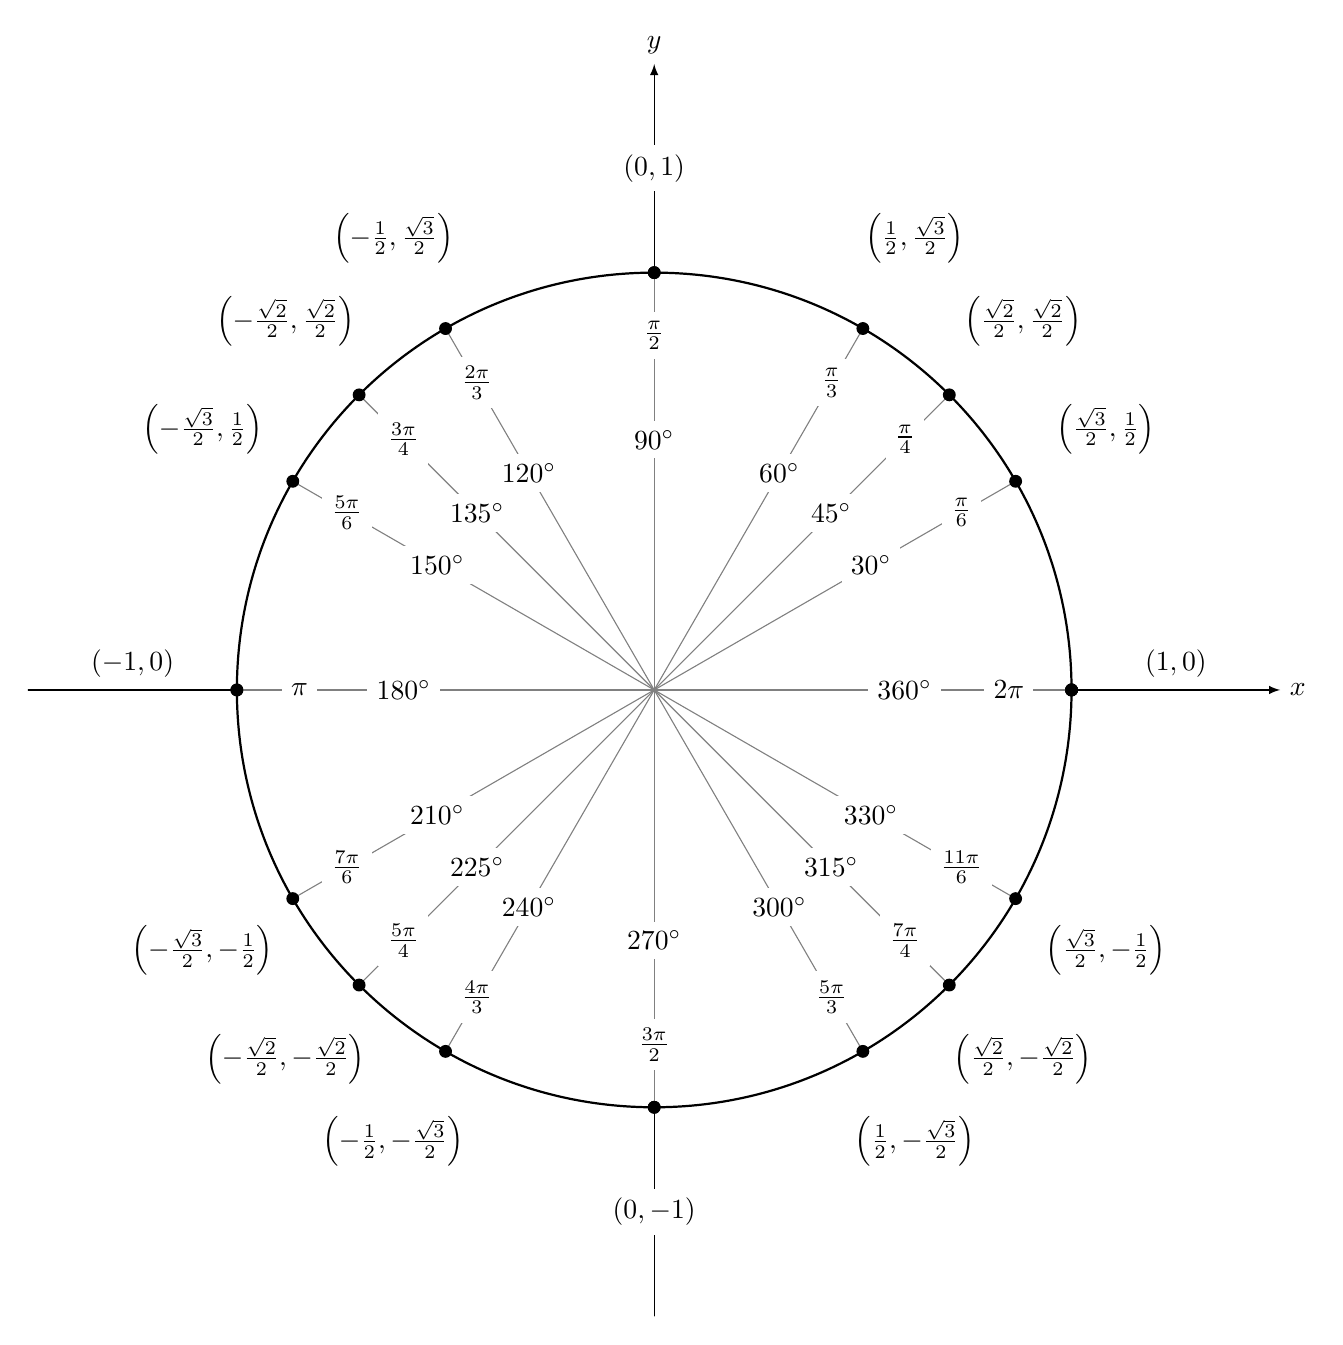
\begin{tikzpicture}[scale=5.3,cap=round,>=latex]
        % draw the coordinates
        \draw[->] (-1.5cm,0cm) -- (1.5cm,0cm) node[right,fill=white] {$x$};
        \draw[->] (0cm,-1.5cm) -- (0cm,1.5cm) node[above,fill=white] {$y$};

        % draw the unit circle
        \draw[thick] (0cm,0cm) circle(1cm);

        \foreach \x in {0,30,...,360} {
                % lines from center to point
                \draw[gray] (0cm,0cm) -- (\x:1cm);
                % dots at each point
                \filldraw[black] (\x:1cm) circle(0.4pt);
                % draw each angle in degrees
                \draw (\x:0.6cm) node[fill=white] {$\x^\circ$};
        }
        
        \foreach \x in {0,45,...,360} {
                % lines from center to point
                \draw[gray] (0cm,0cm) -- (\x:1cm);
                % dots at each point
                \filldraw[black] (\x:1cm) circle(0.4pt);
                % draw each angle in degrees
                \draw (\x:0.6cm) node[fill=white] {$\x^\circ$};
        }
        % draw each angle in radians
        \foreach \x/\xtext in {
            30/\frac{\pi}{6},
            45/\frac{\pi}{4},
            60/\frac{\pi}{3},
            90/\frac{\pi}{2},
            120/\frac{2\pi}{3},
            135/\frac{3\pi}{4},
            150/\frac{5\pi}{6},
            180/\pi,
            210/\frac{7\pi}{6},
            225/\frac{5\pi}{4},
            240/\frac{4\pi}{3},
            270/\frac{3\pi}{2},
            300/\frac{5\pi}{3},
            315/\frac{7\pi}{4},
            330/\frac{11\pi}{6},
            360/2\pi}
                \draw (\x:0.85cm) node[fill=white] {$\xtext$};

        \foreach \x/\xtext/\y in {
            % the coordinates for the first quadrant
            30/\frac{\sqrt{3}}{2}/\frac{1}{2},
            45/\frac{\sqrt{2}}{2}/\frac{\sqrt{2}}{2},
            60/\frac{1}{2}/\frac{\sqrt{3}}{2},
            % the coordinates for the second quadrant
            150/-\frac{\sqrt{3}}{2}/\frac{1}{2},
            135/-\frac{\sqrt{2}}{2}/\frac{\sqrt{2}}{2},
            120/-\frac{1}{2}/\frac{\sqrt{3}}{2},
            % the coordinates for the third quadrant
            210/-\frac{\sqrt{3}}{2}/-\frac{1}{2},
            225/-\frac{\sqrt{2}}{2}/-\frac{\sqrt{2}}{2},
            240/-\frac{1}{2}/-\frac{\sqrt{3}}{2},
            % the coordinates for the fourth quadrant
            330/\frac{\sqrt{3}}{2}/-\frac{1}{2},
            315/\frac{\sqrt{2}}{2}/-\frac{\sqrt{2}}{2},
            300/\frac{1}{2}/-\frac{\sqrt{3}}{2}}
                \draw (\x:1.25cm) node[fill=white] {$\left(\xtext,\y\right)$};

        % draw the horizontal and vertical coordinates
        % the placement is better this way
        \draw (-1.25cm,0cm) node[above=1pt] {$(-1,0)$}
              (1.25cm,0cm)  node[above=1pt] {$(1,0)$}
              (0cm,-1.25cm) node[fill=white] {$(0,-1)$}
              (0cm,1.25cm)  node[fill=white] {$(0,1)$};
    \end{tikzpicture}




\newpage


\thispagestyle{empty}


\setlength\fboxrule{2pt}\setlength\fboxsep{2mm}
\fbox{This page is intentionally left blank.} You may use it as scrap paper for your calculations.
\end{document}                 